\documentclass[12pt]{article}
\usepackage[utf8]{inputenc}
\usepackage[T1]{fontenc}
\usepackage{amsmath}
\usepackage{amsfonts}
\usepackage{amssymb}
\usepackage[version=4]{mhchem}
\usepackage{stmaryrd}
\usepackage{bbold}
\usepackage{hyperref}
\usepackage{graphicx}
\graphicspath{{../data/}}

\usepackage{listings} % Required for insertion of code
\usepackage{xcolor} % Required for custom colors

% Define custom colors
\definecolor{codegreen}{rgb}{0,0.6,0}
\definecolor{codegray}{rgb}{0.5,0.5,0.5}
\definecolor{codepurple}{rgb}{0.58,0,0.82}
\definecolor{backcolour}{rgb}{0.95,0.95,0.92}

% Setup the style for code listings
\lstdefinestyle{mystyle}{
    backgroundcolor=\color{backcolour},   
    commentstyle=\color{codegreen},
    keywordstyle=\color{magenta},
    numberstyle=\tiny\color{codegray},
    stringstyle=\color{codepurple},
    basicstyle=\ttfamily\footnotesize,
    breakatwhitespace=false,         
    breaklines=true,                 
    captionpos=b,                    
    keepspaces=true,                 
    numbers=left,                    
    numbersep=5pt,                  
    showspaces=false,                
    showstringspaces=false,
    showtabs=false,                  
    tabsize=2
}

% Activate the style
\lstset{style=mystyle}

\hypersetup{colorlinks=true, linkcolor=blue, filecolor=magenta, urlcolor=cyan,}
\urlstyle{same}

\title{Assignment 1: Exact diagonalization and quantum phase transitions }


\author{Instructor: Lesik Motrunich\\
TA: Liam O'Brien}
\date{}


\begin{document}
\maketitle
Ph 121C: Computational Physics Lab, Spring 2024

California Institute of Technology

Due: Tuesday, April 16, 2024







\section*{4 Assignment: ED study of quantum Ising model}
For simplicity, in the following we set the parameter $J=1$ in (4) and vary $h$.









\subsection*{4.3 Study of convergence with system size}
For representative values of $h$ inside each phase (e.g., $h=0.3$ in the ferromagnetic phase and $h=1.7$ in the paramagnet), study the $L$ dependence of the ground state energy per site, $E_{\mathrm{gs}}(L) / L$, for systems with both periodic and open boundary conditions. Comment on the approach to the thermodynamic limit $L \rightarrow \infty$ for the two types of boundaries.



It should be clear that periodic boundaries are preferred in order to minimize finite-size effects. However, sometimes open boundary conditions are preferred for technical reasons. An important example is the tensor network representation we will implement later in the course. One can mitigate the effects of the boundaries and better estimate the bulk energy per site using the following trick: for the system with open boundary conditions, plot the values $[E(L=10)-E(L=8)] / 2$, $[E(L=12)-E(L=10)] / 2$, etc. These quantities can be thought of as ground state energy per site for the two sites added in the middle, which feel reduced boundary effects.
\subsubsection{Answer}
As can be seen from the plots the bulk energy density per site converges to a value as the system size increases. These plots use the open boundary conditions.
\begin{figure}
\centering
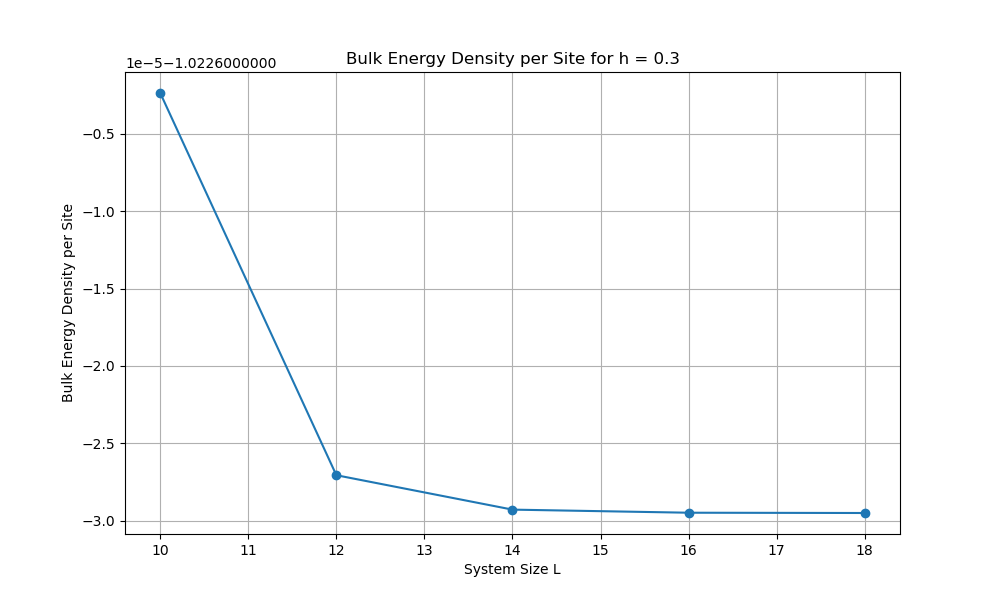
\includegraphics[width=\textwidth]{bulk_energy_density_h0.3.png}
\label{fig:bulk_energy_density}
\end{figure}
\begin{figure}
\centering
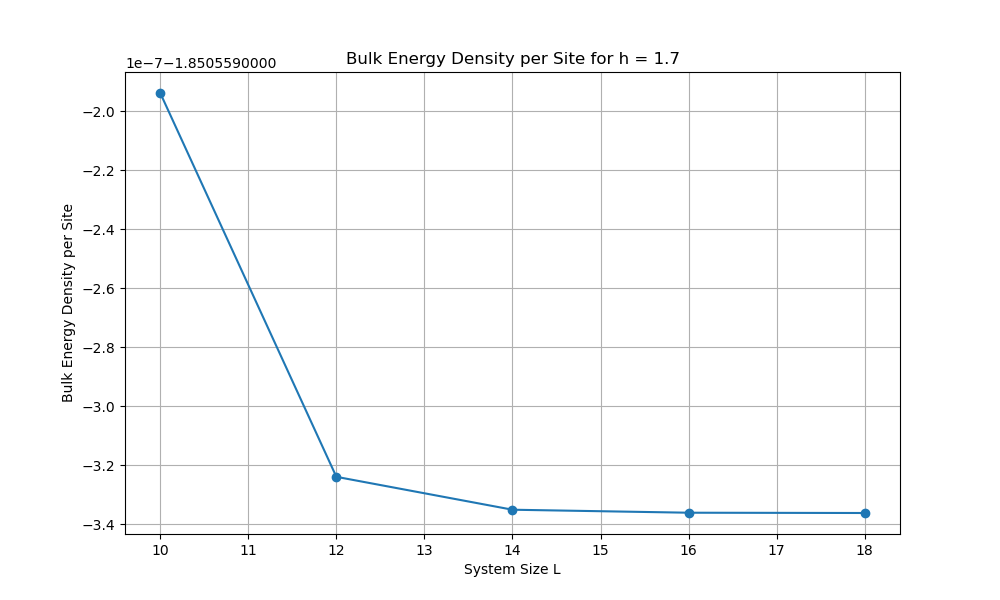
\includegraphics[width=\textwidth]{bulk_energy_density_h1.7.png}
\end{figure}
% Inline Python code in the document
% Inline Python code in the document
\begin{lstlisting}[language=Python]
h_values = [0.3, 1.7]
L_range = range(8, 20, 2)  # From L=8 to L=18, in steps of 2

# Dictionary to store energies for each h value
energies_per_h = {h: [] for h in h_values}

for L in L_range:
    for h in h_values:
        H_open = sparse_hamiltonian(L, h, periodic=False).asformat('csr')
        E_open = scipy.sparse.linalg.eigsh(H_open, k=1, which='SA', return_eigenvectors=False)[0]
        energies_per_h[h].append((L, E_open))

# Now, plot the energy differences for each h value
for h in h_values:
    plt.figure(figsize=(10, 6))
    plt.title(f'Bulk Energy Density per Site for h = {h}')
    Ls, Es = zip(*energies_per_h[h])  # Unpack the energies and L values
    # Calculate the differences and plot
    energy_differences = [(Es[i] - Es[i-1]) / 2 for i in range(1, len(Es))]
    plt.plot(Ls[1:], energy_differences, 'o-', label=f'h = {h}')

    plt.xlabel('System Size L')
    plt.ylabel('Bulk Energy Density per Site')
    plt.grid(True)
    plt.savefig(f'bulk_energy_density_h{h}.png')
\end{lstlisting}
\newpage
\begin{figure}[h]
\centering
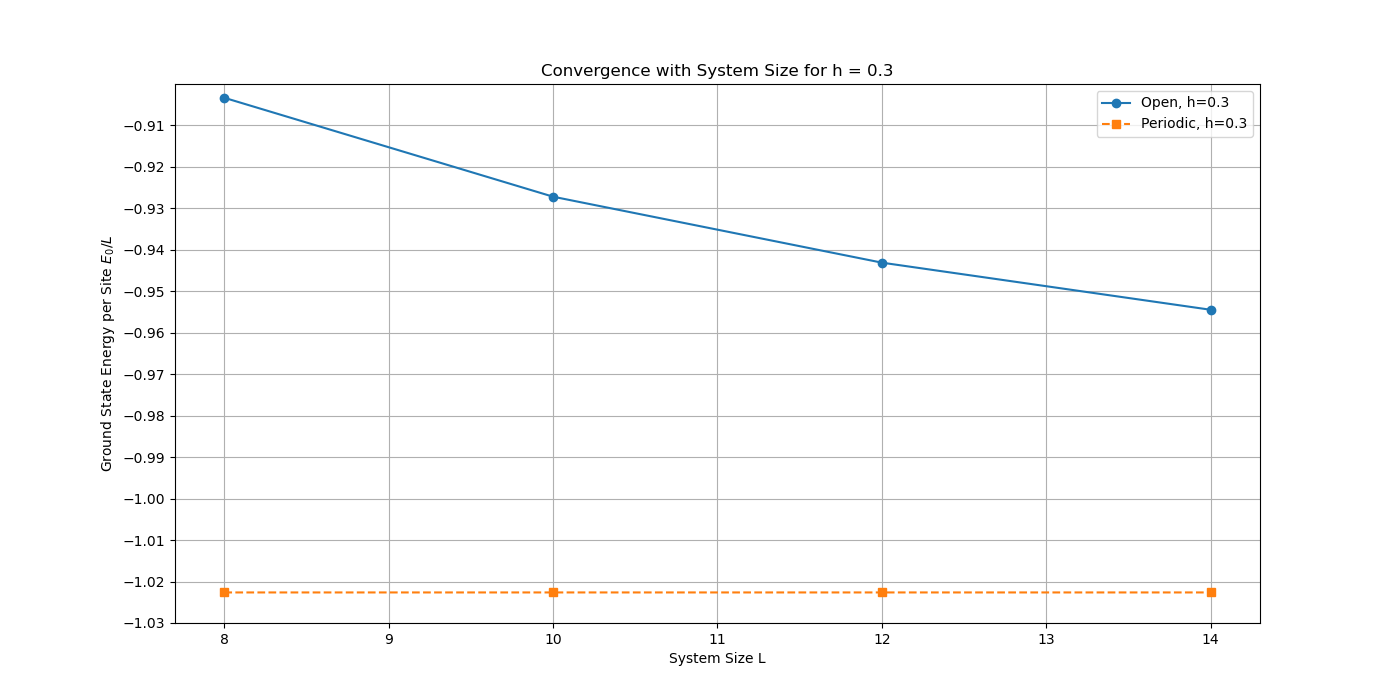
\includegraphics[width=\textwidth]{convergence_h0.3.png}
\end{figure}
\begin{figure}[h]
\centering
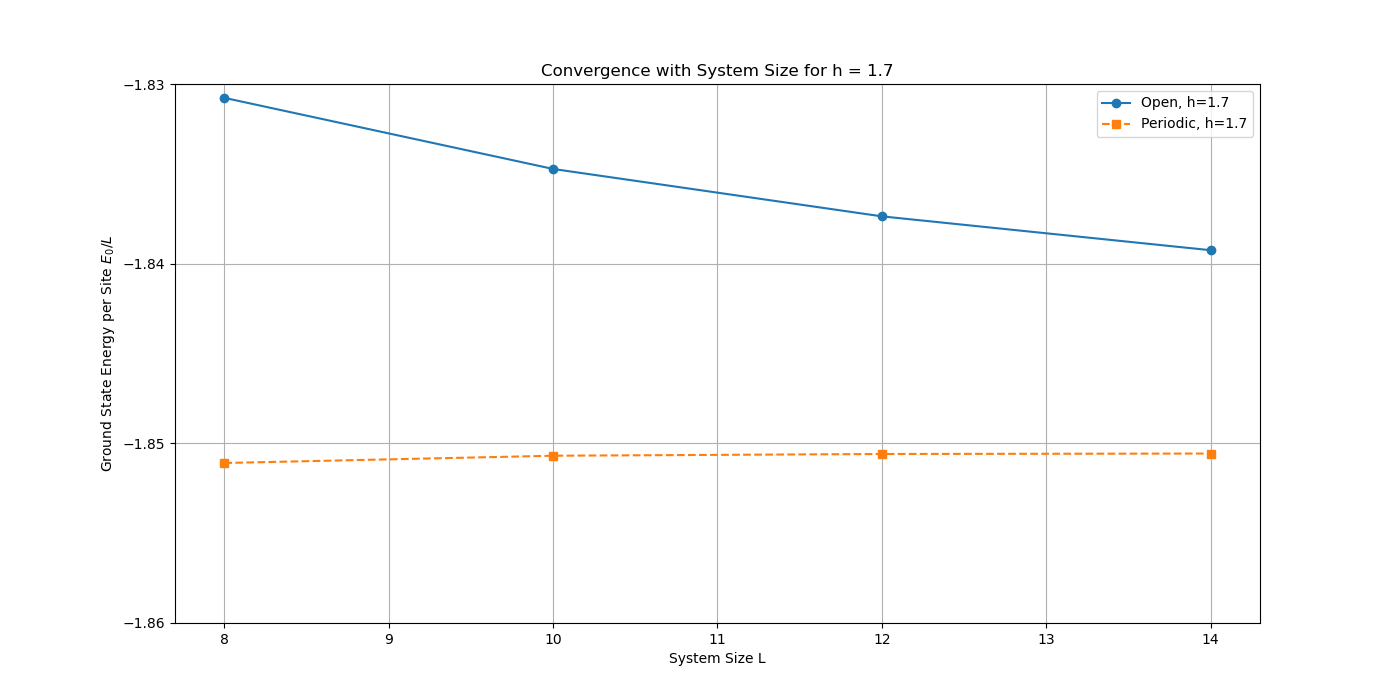
\includegraphics[width=\textwidth]{convergence_h1.7.png}
\end{figure}

Both types of boundaries approach a thermodynamic limit as the system size increases. That is, the periodic systems should be more accurate, but this doesn't matter so much in the thermodynamic limit. One also notices in the convergence plots that when we have a small transverse field $h$, the interaction terms dominate, so the finite size effect is quite pronounced, but this is not the case when we have the larger value for $h$. This can be especially noticed by the fact that the ticks on the vertical axes have the same scaling, but the low $h$ encompasses a much greater number of ticks in its approach towards the thermodynamic limit than the high $h$ case.
% Inline Python code in the document
\begin{lstlisting}[language=Python]
# Representative values of h
h_values = [0.3, 1.7]
# Range of L values to study
L_range = range(8, 16, 2)  # Example: from 8 to 16, in steps of 2

# Initialize storage for energies
energies = {'open': {}, 'periodic': {}}

# Define a consistent interval for y-axis ticks
tick_interval = 0.01  # Adjust this based on the expected range of energy values

for h in h_values:
    energies['open'][h] = []
    energies['periodic'][h] = []

    for bc in ['open', 'periodic']:
        for L in L_range:
            H = sparse_hamiltonian(L, h, periodic=(bc == 'periodic')).asformat('csr')
            energy_per_site = scipy.sparse.linalg.eigsh(H, k=1, which='SA', return_eigenvectors=False)[0] / L
            energies[bc][h].append(energy_per_site)

    # Plotting after collecting all data for the current h
    plt.figure(figsize=(14, 7))
    plt.plot(list(L_range), energies['open'][h], 'o-', label=f'Open, h={h}')
    plt.plot(list(L_range), energies['periodic'][h], 's--', label=f'Periodic, h={h}')

    plt.xlabel('System Size L')
    plt.ylabel('Ground State Energy per Site $E_0 / L$')
    plt.title(f'Convergence with System Size for h = {h}')
    plt.legend()
    plt.grid(True)

    # Determine the min and max energies for this plot to set y-limits appropriately
    min_energy = min(energies['open'][h] + energies['periodic'][h])
    max_energy = max(energies['open'][h] + energies['periodic'][h])

    # Set y-axis limits based on the smallest and largest energies, adjusted to the nearest tick
    plt.ylim((min_energy // tick_interval * tick_interval, 
              (max_energy // tick_interval + 1) * tick_interval))
    plt.yticks(np.arange(min_energy // tick_interval * tick_interval, 
                         (max_energy // tick_interval + 1) * tick_interval, 
                         tick_interval))

    plt.savefig(f'convergence_h{h}.png')
\end{lstlisting}






\subsection*{4.7 Making use of Ising symmetry}
In the previous steps, no use has been made of the Ising symmetry: the fact that unitary $U_{x}=\prod_{j} \sigma_{j}^{x}$ commutes with the Hamiltonian. Correctly implementing the symmetry reduces the size of the diagonalization problem by a factor of two, which saves memory and gives a fourfold speedup.

Set up a sparse diagonalization of the Ising Hamiltonian in the $\sigma^{x}$ basis, utilizing the Ising symmetry as described in Sec. 3.4. As you will no longer be able to exploit the convenient basis (1), the bookkeeping is more challenging here. Obtain a few states in each sector and compare with your previous results. Use the symmetric solver to add a single site to the largest size you were able to solve previously and find the ground state and a few excited states at this size for representative values of $h$ in each phase.

Utilizing symmetries can also improve the accuracy of certain interesting features of the spectrum. For example, in Sec. 2.3 the two ground states in the ordered phase are described as having an energy splitting that is exponentially small in system size. By solving for the ground state within each symmetry sector, try to obtain the dependence of this splitting on system size $L$.
\newpage
\subsubsection{Answer}
As can be seen in figures like \ref{fig:4-6_L12_energy} there is a near exact matching of energies obtained from the symmetric solver and the non-symmetric solver.
\begin{figure}[h]
\centering
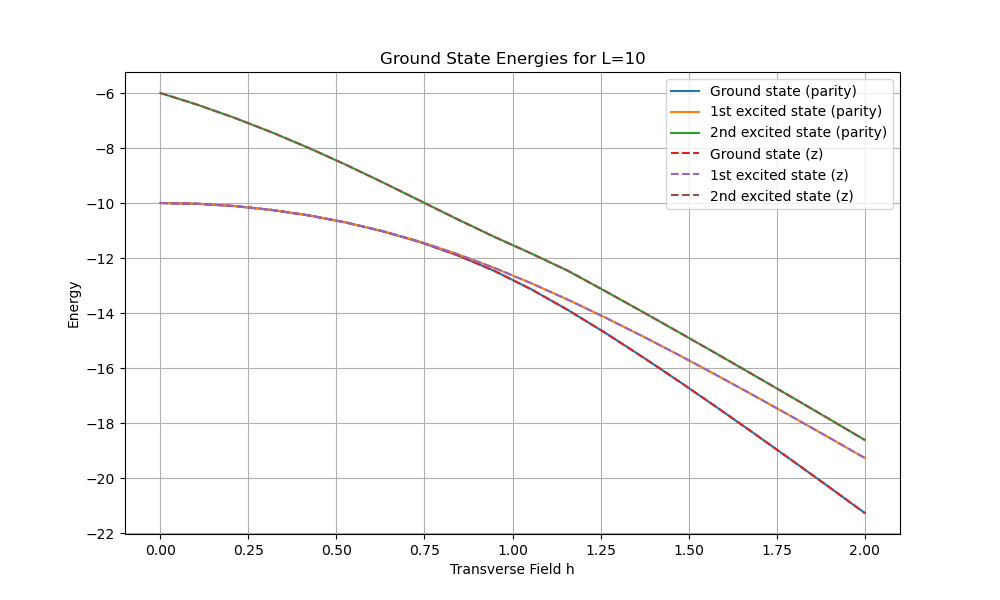
\includegraphics[width=\textwidth]{4-6_L10_energies.png}
\label{fig:4-6_L12_energy}
\end{figure}
% Inline Python code in the document
\begin{lstlisting}[language=Python]
def sparse_hamiltonian_x_basis(L, h, J=1, periodic=False):
    size = 2**L
    index_even = []  # To track indices of even parity states
    index_odd = []   # To track indices of odd parity states

    # Initialize lists for even and odd parity sectors
    row_even, col_even, data_even = [], [], []
    row_odd, col_odd, data_odd = [], [], []

    def count_ones(n):
        """Helper function to count '1's in binary representation."""
        return bin(n).count('1')
    # Populate even and odd indices
    for i in range(size):
        if count_ones(i) % 2 == 0:
            index_even.append(i)
        else:
            index_odd.append(i)

    # Map original indices to new compacted indices
    map_even = {idx: n for n, idx in enumerate(index_even)}
    map_odd = {idx: n for n, idx in enumerate(index_odd)}

    # Construct the Hamiltonian for each state
    for i in range(size):
        x_basis_state = binary_string(i, L)
        parity = count_ones(i) % 2  # Calculate parity of the state

        # Select the correct lists and mapping based on the parity
        row = row_even if parity == 0 else row_odd
        col = col_even if parity == 0 else col_odd
        data = data_even if parity == 0 else data_odd
        mapping = map_even if parity == 0 else map_odd

        # Diagonal contributions from ^x (magnetic field)
        row.append(mapping[i])
        col.append(mapping[i])
        data.append(-h * (x_basis_state.count('1') - x_basis_state.count('0')))

        # Off-diagonal contributions from ^z ^z interaction
        loop_range = L if periodic else L - 1
        for j in range(loop_range):
            flipped_index = i ^ (1 << j) ^ (1 << ((j + 1) % L))
            if flipped_index in mapping:  # Check if flipped index is in the same parity
                row.append(mapping[i])
                col.append(mapping[flipped_index])
                data.append(-J)

    # Create sparse matrices for each parity sector
    H_even = sp.coo_matrix((data_even, (row_even, col_even)), shape=(len(index_even), len(index_even)), dtype=float).tocsr()
    H_odd = sp.coo_matrix((data_odd, (row_odd, col_odd)), shape=(len(index_odd), len(index_odd)), dtype=float).tocsr()

    return H_even, H_odd

# Example usage:
L = [8, 10, 12]
h_values = np.linspace(0, 2.0, 20)  # Range of h values to scan

for L_val in L:
    plt.figure(figsize=(10, 6))
    plt.title(f'Ground State Energies for L={L_val}')
    
    # Lists to store the lowest three unique energies for each h value
    lowest_three_parity = []
    lowest_three_z_basis = []

    for h_val in h_values:
        H_even, H_odd = sparse_hamiltonian_x_basis(L_val, h_val, periodic=True)
        H_z = sparse_hamiltonian(L_val, h_val, periodic=True)

        # Diagonalize and collect the lowest three energies for even sector
        eigvals_even = scipy.sparse.linalg.eigsh(H_even, k=3, which='SA', return_eigenvectors=False)
        
        # Diagonalize and collect the lowest three energies for odd sector
        eigvals_odd = scipy.sparse.linalg.eigsh(H_odd, k=3, which='SA', return_eigenvectors=False)
        
        # Combine and sort the eigenvalues from even and odd sectors, then take the lowest three
        combined_parity_eigvals = np.union1d(eigvals_even, eigvals_odd)
        combined_parity_eigvals.sort()
        
        # Append to the list of lowest three energies for the parity sectors
        lowest_three_parity.append(combined_parity_eigvals[:3])

        # Diagonalize and collect the lowest four energies for the z-basis for comparison
        eigvals_z = scipy.sparse.linalg.eigsh(H_z, k=4, which='SA', return_eigenvectors=False)
        eigvals_z.sort()

        # Append to the list of lowest three energies for the z-basis
        lowest_three_z_basis.append(eigvals_z[:3])

    # Reshape the lists for plotting
    lowest_three_parity = np.array(lowest_three_parity).T  # Transpose to match h_values shape
    lowest_three_z_basis = np.array(lowest_three_z_basis).T

    # Plot for parity sectors
    plt.plot(h_values, lowest_three_parity[0], label='Ground state (parity)')
    plt.plot(h_values, lowest_three_parity[1], label='1st excited state (parity)')
    plt.plot(h_values, lowest_three_parity[2], label='2nd excited state (parity)')

    # Plot for z-basis; using dashed lines for distinction
    plt.plot(h_values, lowest_three_z_basis[0], label='Ground state (z)', linestyle='--')
    plt.plot(h_values, lowest_three_z_basis[1], label='1st excited state (z)', linestyle='--')
    plt.plot(h_values, lowest_three_z_basis[2], label='2nd excited state (z)', linestyle='--')

    plt.xlabel('Transverse Field h')
    plt.ylabel('Energy')
    plt.legend()
    plt.grid(True)
    plt.savefig(f'4-6_L{L_val}_energies.png')  
\end{lstlisting}
We also did this for L=21 in \ref{4-6_parity_resolved_energies.png}.
\begin{figure}[h]
\centering
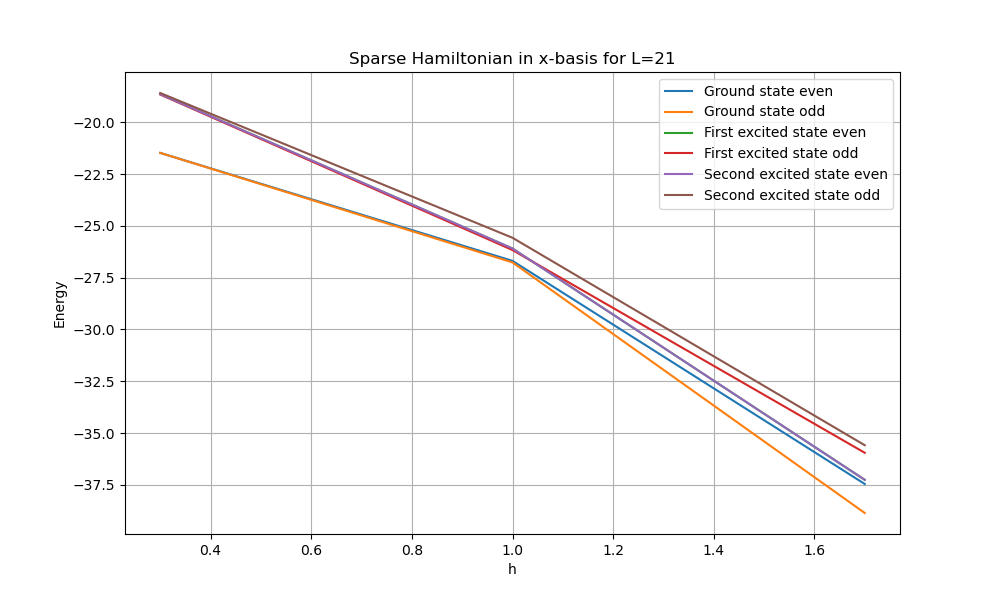
\includegraphics[width=\textwidth]{4-6_parity_resolved_energies.png}
\label{4-6_parity_resolved_energies.png}
\end{figure}
% Inline Python code in the document
% Inline Python code in the document
% Inline Python code in the document
\begin{lstlisting}[language=Python]
L = 21
h_vals = [0.3, 1, 1.7]  # This should probably be h_vals to avoid confusion with h in plt.plot
energies_ground_even = []
energies_ground_odd = []
energies_first_excited_even = []
energies_first_excited_odd = []
energies_second_excited_even = []
energies_second_excited_odd = []

plt.figure(figsize=(10, 6))
plt.title(f'Sparse Hamiltonian in x-basis for L={L}')
for h_val in h_vals:
    H_even, H_odd = sparse_hamiltonian_x_basis(L, h_val, periodic=True)
    eigvals_even, _ = scipy.sparse.linalg.eigsh(H_even, k=3, which='SA')
    eigvals_odd, _ = scipy.sparse.linalg.eigsh(H_odd, k=3, which='SA')
    
    energies_ground_even.append(eigvals_even[0])
    energies_ground_odd.append(eigvals_odd[0])

    energies_first_excited_even.append(eigvals_even[1])
    energies_first_excited_odd.append(eigvals_odd[1])

    energies_second_excited_even.append(eigvals_even[2])
    energies_second_excited_odd.append(eigvals_odd[2])

# Now plot using the accumulated lists
plt.plot(h_vals, energies_ground_even, label='Ground state even')
plt.plot(h_vals, energies_ground_odd, label='Ground state odd')
plt.plot(h_vals, energies_first_excited_even, label='First excited state even')
plt.plot(h_vals, energies_first_excited_odd, label='First excited state odd')
plt.plot(h_vals, energies_second_excited_even, label='Second excited state even')
plt.plot(h_vals, energies_second_excited_odd, label='Second excited state odd')

plt.xlabel('h')
plt.ylabel('Energy')
plt.legend()
plt.grid(True)
plt.savefig('4-6_parity_resolved_energies.png')

\end{lstlisting}
Then we made a plot for the splitting as a function of system size in the ferromagnet. From the perturbation theory, it can be derived that the energy splitting goes as $\left(\frac{h}{J}\right)^L$. But since we have $\frac{h}{J}<1$ with $h=0.3$ and $J=1$, the splitting will be exponentially small in the system size.
\begin{figure}[h]
\centering
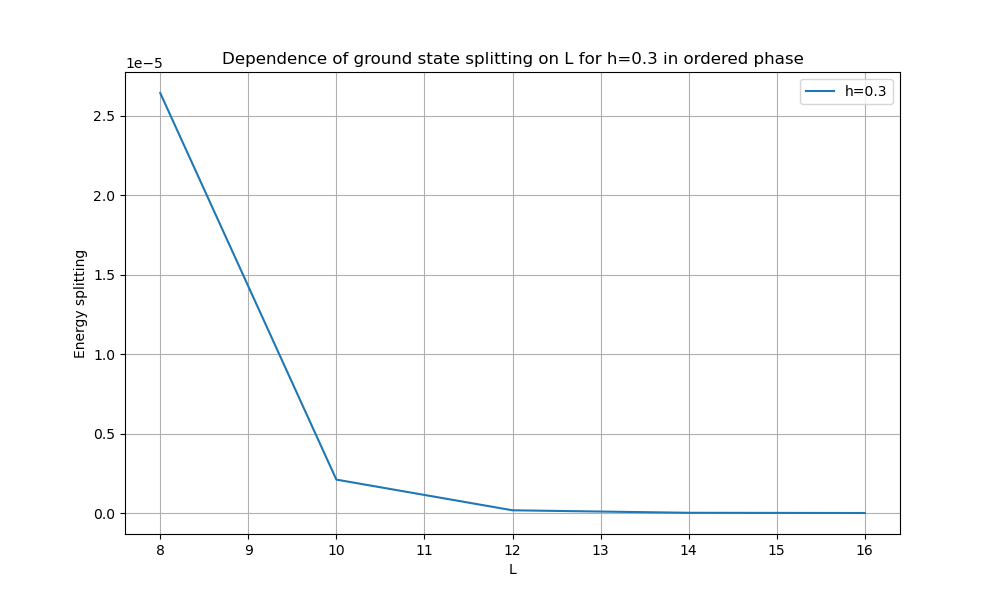
\includegraphics[width=\textwidth]{4-6_L_dependence.png}
\label{4-6_L_dependence.png}
\end{figure}
% Inline Python code in the document
\begin{lstlisting}[language=Python]
L =[8, 10, 12, 14, 16]
h = 0.3
plt.figure(figsize=(10, 6))
plt.title(f'Dependence of ground state splitting on L for h={h} in ordered phase')
energies = []
excitation_energy = []
for L_val in L:
    H_even, H_odd = create_sparse_hamiltonian_x_basis(L_val, 1, h)
    eigvals_even, _ = scipy.sparse.linalg.eigsh(H_even, k=2, which='SA')
    eigvals_odd, _ = scipy.sparse.linalg.eigsh(H_odd, k=2, which='SA')
    # append all of the energies to a list
    energies.append([eigvals_even[0], eigvals_odd[0]])
    # energies.append([eigvals_even[1], eigvals_odd[1]])
    energies.sort()
    # determine the excitation energy
    excitation_energy.append(energies[0][1] - energies[0][0])

# fought the excitation and energy for each the value of L
plt.plot(L, excitation_energy, label=f'h={h}')
plt.xlabel('L')
plt.ylabel('Energy splitting')
plt.legend()
plt.grid(True)
plt.savefig('4-6_L_dependence.png')
\end{lstlisting}
\newpage





\section*{References}
[1] Sandvik, Anders W. "Computational studies of quantum spin systems." In AIP Conference Proceedings, vol. 1297, no. 1, pp. 135-338. American Institute of Physics, 2010.

[2] Golub, Gene H., and Charles F. van Loan. Matrix computations. Vol. 3. JHU press, 2013.

[3] \href{https://en.wikipedia.org/wiki/Bitwise_operation}{https://en.wikipedia.org/wiki/Bitwise\_operation}

[4] \href{https://docs.scipy.org/doc/scipy/reference/sparse.html}{https://docs.scipy.org/doc/scipy/reference/sparse.html}


\end{document}